\documentclass[12pt,a4paper]{book} % 12pt font size, A4 paper and two-sided margins twocolumn,oneside

\usepackage[a4paper,text={16.5cm,25.2cm},centering]{geometry}
\makeatletter				% pour faire de @ une lettre simple (et non un caractère associé à une macro interne
\usepackage{amsmath,amsthm,amsfonts,amssymb,mathtools}
\usepackage{color,graphicx,xcolor}
\usepackage{tikz}
\usetikzlibrary{decorations.pathreplacing}
\usepackage[prefix=rt]{xcolor-material}

\usepackage{multicol}			% pour mettre un \begin{multicols}...\end{multicols} et faire du multicolonnage localement dans une page
 
%XeLaTeX is essentially a replacement for pdfLaTeX. It was primarily developed to enable better font handling. For latin writers, the main benefit of XeLaTeX is the ability to use the fonts on your computer, just as you can with other software.
\usepackage{fontspec,xltxtra,xunicode}
\defaultfontfeatures{}
%\usepackage{palatino} % Use the Palatino font
% to choose a font, you just need its full name on your system
% fc-list  | grep -i texgyr
% Here, the scales of the fonts have been chosento equalise their lowercase letter heights
\setmainfont{TeX Gyre Adventor}[Scale=MatchLowercase]
\usepackage{makeidx}			% pour permettre de construire un index

\usepackage{fancybox}			% pour faire des boites entourée de différents types de cadres
\usepackage{framed}			% pour mettre des sortes de minipages encadrées sur plusieures pages, sur fond coloré
\usepackage{boxedminipage}		% pour mettre des bordures aux minipages
\usepackage{relsize,fancyvrb}		% pour mettre des textes non interprétés encadrés et changer la taille des caractères à l'intérieur

\usepackage{lettrine}			% pour mettre des lettrines
\usepackage{listings}			% pour mettre du code informatique non interprété
\usepackage[shellescape,latex]{gmp}
\usepackage{mpgraphics}
\usepackage{caption}			% pour gérer encore mieux les légendes
\makeatother				% pour refaire de @ une lettre différente des autres (exploitée dans des macros)

\renewcommand{\captionfont}{\it \small}	% pour avoir de l'italique pour le texte de légende
\renewcommand{\captionlabelfont}{\it \bf \small}
\DeclareCaptionLabelSeparator{endash}{ -- }	% pour définir un tiret après le numéro des légentes
\captionsetup{labelsep=endash,justification=centering,belowskip=10pt}	% pour avoir un petit trait après le no de légende

\lstdefinestyle{hama}{%
    literate={1}{\raisebox{0.5ex}{\fbox{\textcolor{blue}{1}}}}{1}%
        {0}{\fbox{\textcolor{red}{0}}}{1},%
    basicstyle=\ttfamily,%
}


\newcommand{\HAMA}[1]{\lstinline[style=hama]{#1}}

\newcommand{\Ra}[1]{\textcolor{rtLightBlue900}R\textsubscript{\textcolor{rtLightBlue900}{#1}}}
\newcommand{\Rab}[1]{\small{\textcolor{rtLightBlue900}{2}}\textcolor{rtLightBlue900}R\textsubscript{\textcolor{rtLightBlue900}{#1}}}
\newcommand{\gd}[1]{\textbf{δ}\textsubscript{\textbf{#1}}}
\newcommand{\gc}[1]{\textbf{γ}\textsubscript{\textbf{#1}}}
\newcommand{\gq}[1]{\textbf{ε}\textsubscript{\textbf{#1}}}
\newcommand{\Ca}[1]{\textcolor{rtLightBlue900}C\textsubscript{\textcolor{rtLightBlue900}{#1}}}
\usepackage{nextpage}							% pour retirer les entêtes de la dernière page vide d'un chapitre ;
\newcommand\myclearpage{\cleartooddpage[\thispagestyle{plain}]}		% il faut ensuite placer \myclearpage à la fin de chaque chapitre.
\def\siecle#1{\textsc{\romannumeral #1}\textsuperscript{e}~siècle}	% macro pour écrire les siècles : \siecle{19} par exemple

\newcommand{\concept}[1]{\textcolor{rtLightBlue900}{#1}} 
\newcommand{\subconcept}[1]{\textcolor{rtLightBlue900}{\textit{#1}}}

%\makeindex				% pour construire effectivement l'index
\begin{document}
\tableofcontents{}

\renewcommand{\listfigurename}{Liste des figures}
\listoffigures

\myclearpage

%\listoftables
%%Text\textsubscript{effect}
\chapter{Introduction}

\lettrine{C}{ette introduction} présente en premier lieu l'incontournable ...\textbf{Giordano Bruno (1548-1600)\index{Bruno Giordano}} \LaTeX{} 





\begin{figure*}[t]
\caption[La taille des planètes]{La queue de la comète\label{billetcomete}}
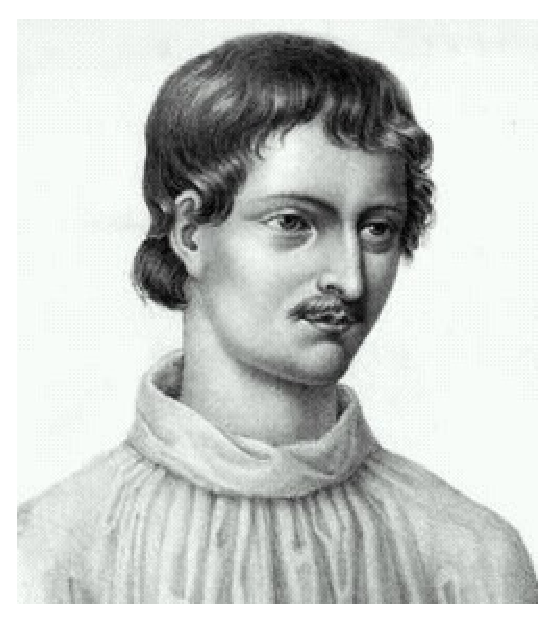
\includegraphics[width=4cm]{Giordano_Bruno.eps}
\end{figure*}

\section{Définitions des expressions mathematiques}


\begin{mpinline}
draw (20,20)--(0,0)--(0,30)--(30,0)--(0,0)
\end{mpinline}

\section{GÉOMÉTROGRAPHIE}

\begin{mpdisplay}
u=1cm;
draw (2u,2u)--(0,0)--(0,3u)--(3u,0)--(0,0);
pickup pencircle scaled 4pt;
for i=0 upto 2:
for j=0 upto 2: drawdot (i*u,j*u); endfor
endfor
\end{mpdisplay}
%\entry{Géométrographie}{définition}{ʒeɔ.me.tʁɔ.ɡʁa.fi}{estArt des constructions géométriques .}

\lettrine{L}{a théorie} proprement dite qui n'est, en somme, que l'indication
de notations avec les conventions adoptées.
\begin{mpost}[name=mwe]
    numeric u; u:=1.0cm;
    draw (0,0)*u--(1,0)*u;
    label(\btex "A" etex, (0,0)*u);
    label(\btex "B" etex, (1,0)*u);
\end{mpost}

\usempost[width=4.0in]{mwe}
\begin{mpost*}
ua:=1;
for i = -.3cm step .6cm until 3.6cm:
    label.bot(decimal ua,(i,-3.7cm));
    ua := incr(ua);
endfor
  % draw a line  
  draw (1cm,2cm) -- (3cm,5cm);     
\end{mpost*}


\subsection{NOTATIONS.}

Une notation géométrographique \emph{Bernes},  \gd{1} \gc{1} \gq{1}.

Une notation géométrographique \emph{Lemoine}, \Ra{1} \Ra{2} \Rab{1} \Ca{1} \Ca{2} \Ca{3}.


\Ra{1} \gd{1} \gc{1} \gq{1}

Symboles pour la règle : \Ra{1} \Ra{2} ou \gd{1} \gd{2}

Tracer une droite quelquonque : \Ra{2}  \gd{}

Faire passer le bord d'une règle par un point placé s'appellera l'\emph{opération} \Ra{1} ou \gd{1}, pour abréger, op.: (\Ra{1} \gd{1}); donc, spéculativement, faire bord d'une règle par deux points sera l'opération: (\Rab{1}  \gd{2}).


Tracer une ligne en suivant le bord de la règle sera (\Ra{2} ou \gd{2}).

Symboles pour le compas : \Ca{1} \gc{1} \Ca{2} \gc{2} \Ca{3}  \gc{}

Tracer un cercle quelquonque : (\Ca{3} \gc{}).


Mettre la pointe du compas en \emph{un point placé} sera op. (\Ca{1} ou \gc{1}); donc, spéculativement prendre avec le compas la distance de deux points placés sera op. (2\Ca{1} \gc{3}).

Tracer un cercle mais dont le centre est soit un point déterminé soit sur une ligne  : (\Ca{2} \gc{2}).




M. Bernes ne fait pas la distinction que j'établis entre (\Ca{1} \Ca{2}). Placer la pointe du compas en un point indéterminé d'une ligne tracée, c'est-a-dire ce que j'appelle \Ca{2}, il l'assimile a
\Ca{1}, c-a-d la pointe en un point déterminé. C'est d'ailleurs
une distinction dont 1 importance n'est que spéculative;


Symboles pour l'équerre :

Parallèle ou perpendiculaire quelconque à la ligne de terre au moyen de l'equerre ou du T : \gq{} .
 
 Ligne de rappel ou parallèle  à la ligne de terre passant par un point déterminé : \gq{1} .
 
Parallèle  quelconque à une droite :\gq{2} .
 
 Parallèle à une droite donnée passant par un point determiné  :\gq{3} .
 
 
 
 \subsection{coefficient de simplicité ou simplicité.}
 Nous supposerons que toute droite tracée et que tout cercle
tracé dans le cours d'une construction le sont en entier.

A la Géométrie canonique des Grecs, qui n'admet que les
solutions par la droite et le cercle, correspondra la Géornétrographie canonique qui admettra seulement la règle et le compas.


une construction ; en notation géométrographique \emph{Lemoine} ;s'exprimera par une formule : 

$[l_{1}.\Ra{1} + l_{2}.\Ra{2} + m_{1}.\Ca{1} + m_{2}.\Ca{2} + m_{3}.\Ca{3}]$.

Le nombre $l_{1} + l_{2}+ m_{1} + m_{2} + m_{3}$ est \emph{le coefficient de simplicité}.

Le nombre $l_{1} +  m_{1} + m_{2}$ est \emph{le coefficient d'exactitude}.

Le nombre $ l_{2}$ correspond au nombre de ligne tracées.

Le nombre $m_{3}$ correspond au nombre de cercles tracés.

une construction ; en notation géométrographique \emph{Bernes}  avec equerre,  \gd{1} \gc{1} \gq{1} ;s'exprimera par une formule : 

$[l.\gd{} + l_{1}.\gd{1} + l_{2}.\gd{2} + m.\gc{} + m_{1}.\gc{1} + m_{2}.\gc{2} + n.\gq{} + n_{1}.\gq{1} + n_{2}.\gq{2} + n_{3}.\gq{3} ]$ 


Le nombre $l + 2.l_{1} + 3.l_{2} + m + 2.m_{1} + 3.m_{2} + 4.m_{3} + n + 2.n_{1} + 3.n_{2} + 4.n_{3}$ est \emph{le coefficient de simplicité}.

Le nombre $l_{1} + 2.l_{2} + m_{1} + 2.m_{2} + 3.m_{3} + n_{1} + 2.n_{2} + 3.n_{3}$ est \emph{le coefficient d'exactitude}.

Le nombre $l + l_{1} + l_{2} + n + n_{1} + n_{2} + n_{3}$ correspond au nombre de ligne tracées.

Le nombre $ m + m_{1} + m_{2} + m_{3}$ correspond au nombre de cercles tracés.


a notation A(ρ) ou A(BC) désignera le cercle de centre A et de rayon ρ ou BC.


Je conviens de définir la simplicité d'une construction par son coeficient de simplicité; la construction géométrographique sera donc celle qui a le coeficient de simplicité le plus petit.




 L'application en discutant les constructions fondamentales classiques qui se trouvent partout
les mêmes, transmises séculairement par les géomètres depuis
les Grecs, dans tous les ouvrages de géométrie.


Je montre ainsi, dès le début, que ces constructions universellement enseignées peuvent, toutes à peu près, être notablement simplifiées, quelquefois dans des proportions qui semblent invraisembables, et que l'on est conduit à la notion d'un Art des constructions géométriques et à une methode pour les simplifier.


%%\appendix

\onecolumn
\section{liste}
Tracer une droite quelconque; op.

Tracer une droite qui passe par un point placé

Tracer une droite passant par deux points placés 
Tracer un cercle quelconque op. (C3).

Tracer un cercle quelconque dont le centre est placé;

VI. Prendre avec le compas une longueur donnée AB
op.
Tracer un cercle dont le rayon est une longueur donnée
et le centre un point place; op. 
VIII. Porter sur une ligne donnée, à partir d'un point indé-
terminé de cette ligne ou à partir d'un point placé
sur cette ligne, la longueur comprise entre les branches du compas

Tracer un angle droit ou tracer deux droites perpendicu-
laires entre elles.
...

\end{document}